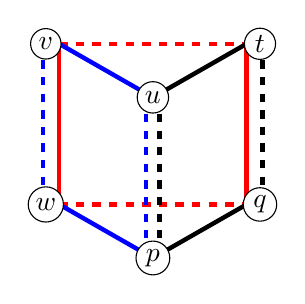
\begin{tikzpicture}[scale=1.7]
 \draw[ultra thick, dashed, red] (0,-.5) -- (1.4,-.5);
 \draw[ultra thick, dashed, red] (0,.7) -- (1.4,.7);
\draw[ultra thick, red] (0,-.5) -- (0,.7);
\draw[ultra thick, red] (1.4,-.5) -- (1.4,.7);
\draw[ultra thick, blue] (0,.7) -- (.7,.3);
\draw[ultra thick, black] (.7,.3) -- (1.4,.7);
\draw[ultra thick, blue] (0,-.5) -- (.7,-.9);
\draw[ultra thick, black] (.7,-.9) -- (1.4,-.5);
\draw[ultra thick, dashed, blue] (.65,.3) -- (.65,-.9);
 \draw[ultra thick, dashed, black] (.75,.3) -- (.75,-.9);
\draw[ultra thick, dashed, blue] (-.12,.7) -- (-.12,-.5);
 \draw[ultra thick, dashed, black] (1.52,.7) -- (1.52,-.5);
\node[circle, fill=white, draw=black, text=black,  inner sep=1.5pt] at (-.1,.7) {$v$};
\node[circle, fill=white, draw=black, text=black,  inner sep=1.5pt] at (.7,.3) {$u$};
\node[circle, fill=white, draw=black, text=black,  inner sep=1.5pt] at (1.5,.7) {$t$};
\node[circle, fill=white, draw=black, text=black,  inner sep=1.5pt] at (-.1,-.5) {$w$};
\node[circle, fill=white, draw=black, text=black,  inner sep=1.5pt] at (0.7,-.9) {$p$};
\node[circle, fill=white, draw=black, text=black,  inner sep=1.5pt] at (1.5,-.5) {$q$};
\end{tikzpicture}
